Wireless Sensor Networks are not yet the ubiquitous tools that help us interact
with the physical world, but they gather more and more deployments, both for
research and business. These deployments vary widely in assumptions and
conditions, as they range from the wireless sensor network put inside a home to
monitor basic parameters, to agricultural WSNs
\cite{burrell2004vineyard,baggio2005wireless} used for fine-grained irrigation
control, to space exploration applications \cite{ulmer2003wireless} etc. All
these applications require different types of interfaces with the rest of the
world and impose restrictions on the gateway/base-station. Current gateway
platforms \cite{hill2004platforms,da2011design,da2011design2} are bulky devices
or PCs connected to one of the wireless nodes that serve as a base-station. We
aim to show in this paper that there exists a solution for gateway design that
is more versatile - can be included in any application -, is smaller and
cheaper and offers ease of use and programming.

We introduce SparrowDongle, a USB stick featuring two microcontrollers that is
designed to be included in wireless networks composed of 2.4GHz Zigbee nodes,
especially our own design, Sparrowv3.2. We will show an overview of the system
architecture in Chapter \ref{chap:arch}, the hardware and software
implementation in Chapter \ref{chap:impl} and results of using the gateway in
Chapter \ref{chap:results}. 

\begin{figure}[ht] \centering
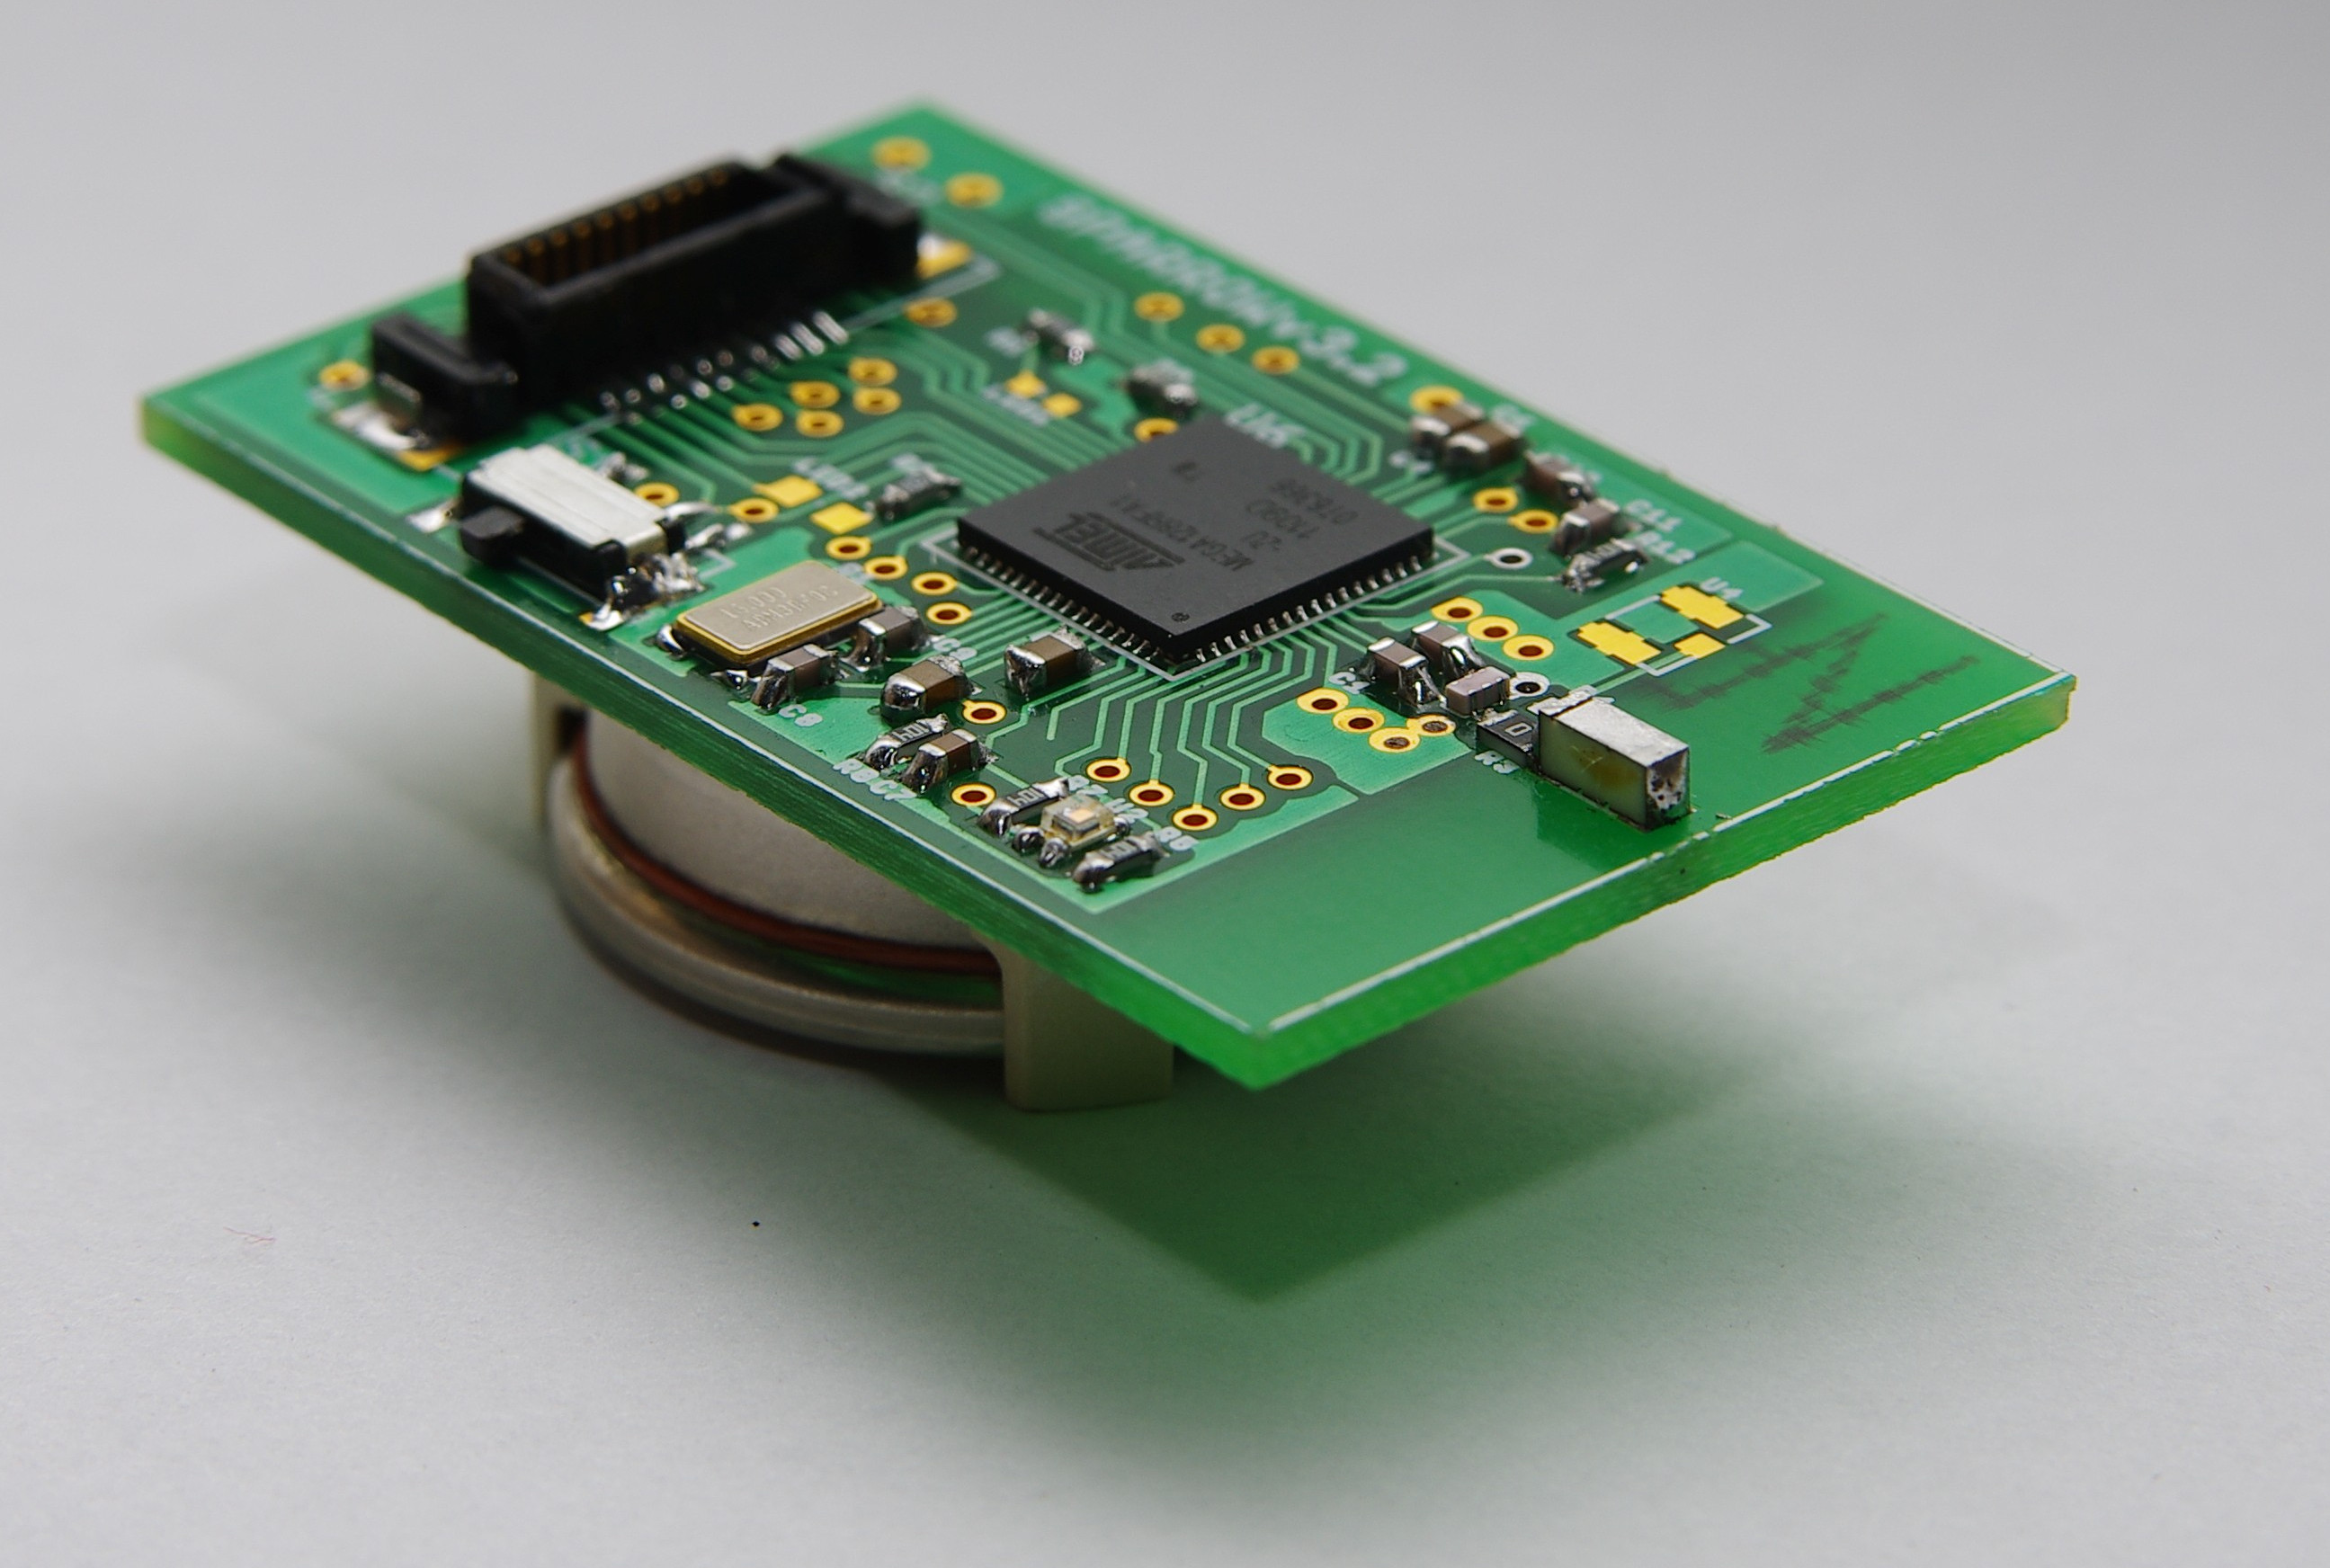
\includegraphics[width=0.4\textwidth]{img/Sparrowv32.jpg} \caption{Sparrow v3.2
wireless node} \end{figure}


